%\begin{frame}
%    \frametitle{Proof of the Lemma}

%    \begin{lemma}
%    	Let a linear system $Ap = b$ from variables
%	    $p = (p_{i, j})_{i \in [m], j \in [n]}$ have $k \le \frac{n - 1}{2}$
%	    equations and have an acceptable solution. Then  $\forall i \in [m] \exists
%        \sigma:$ $\sigma$ is an acceptable solution and satisfies $p_{i, 1} \lor
%        p_{i, 2} \lor \dots \lor p_{i,n}$.
%    \end{lemma}
    
%    \pause
%	\begin{itemize}
%		\item $1 \to 0$ can't violate the acceptability.
%    	\pause
%		\item Let $\pi$ be acceptable solution with the minimal number of 1's.
%	    \pause
%		\item $\pi$ contains at most $k$ ones.
%	    	\pause
%			\begin{itemize}
%				\item Variables with value $1$ in $\pi$: $p_{j_1}, p_{j_2}, \dots,
%	                p_{j_{k + 1}}$ 
%				\item $\exists \tau \neq 0: A \tau = 0$ and support of $\tau$ is in
%		            $p_{j_1}, p_{j_2}, \dots, p_{j_{k + 1}}$. 
%				\item $A(\pi + \tau) = b$, $\pi + \tau$ is acceptable.
%			\end{itemize}
%        \pause
%		\item $\pi$ has $k + 1$ empty holes with numbers $\ell_1, \ell_2, \dots,
%   		\ell_{k + 1}$
%        \pause
%		\item $\exists \tau \neq 0: A \tau = 0$ and support of $\tau$ is in
%    		$p_{i, \ell_1}, p_{i, \ell_2}, \dots, p_{i, \ell_{k + 1}}$.
%		\item $A(\pi + \tau) = b$, $\pi + \tau$ is acceptable and satisfies $p_{i, 1}
%		    \lor p_{i, 2} \lor \dots \lor p_{i,n}$.
%	\end{itemize}
%\end{frame}



\begin{frame}
    \frametitle{Lower bound for 2-fold Tseitin formulas}

    \begin{itemize}
		\item For unsatisfiable $\phi$ a search problem $Search_\phi$: find a
		    falsified clause given a variable assignment.  
		\item We prove that it is possible to transform a splitting tree $T$ into a
		    randomized communication protocol for the problem $Search_\phi$ of depth
	        $O(\log |T| \log\log |T|)$ if some variables are known by Alice and other
	        variables are known by Bob.
		\item Use a lower bound on the randomized communication complexity of the
		    problem $Search_{TS^2_{G,c}}$ for a 2-fold Tseitin formula $TS^2_{G,c}$
            that follows from [Kalyanasundaram, Schintger 1992] and
            [Beame, Pitassi, Segerlind, 2007].
	\end{itemize}
	\pause
    \begin{theorem}
        In time polynomial in $n$ one may construct a graph $G(V, E)$ on $n$ vertices
        with maximal degree bounded by a constant and a function $c: V \to
        \mathbb{F}_2$ such that the size of any linear splitting tree of
        $TS^2_{(G,c)}$ is at least $\Omega\left(2^{n^{1 / 3} / \log^3(n)} \right)$.
    \end{theorem}
\end{frame}



\begin{frame}
    \frametitle{Res-Lin}

    \begin{itemize}
		\item Literal: $L = x_{1} + x_{2} + \dots + x_{k} = \alpha$,
    		$\lnot L = x_{1} + x_{2} + \dots + x_{k} = \alpha + 1$
		\item Linear clause: $\bigvee_i x_{i, 1} + x_{i, 2} + \dots + x_{i, k_i} =
		    \alpha_i$ or $\lnot \bigwedge x_{i, 1} + x_{i, 2} + \dots + x_{i, k_i} =
            1 + \alpha_i$.
        \pause
		\item Res-Lin:
			\begin{itemize}
				\item Resolution rule: $\frac{(f = 0) \lor D, (f = 1) \lor D'}
            		{D \lor D'}$ 
				\item Weakening rule: $\frac{C}{C'}$ if $C$ semantically implies $C'$
			\end{itemize}
		\item \mycolor{blue}{Tree-like} Res-Lin is equivalent to LST.
	\end{itemize}
	\only<2>{\scalebox{0.8}{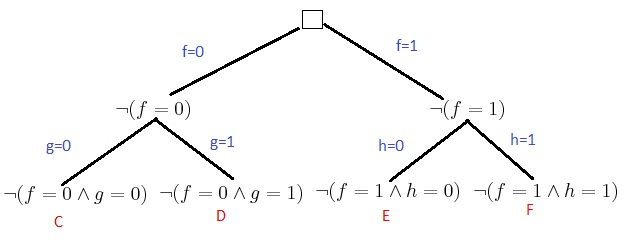
\includegraphics{pics/resdpll.jpg}}}
\end{frame}



\begin{frame}
    \frametitle{Res-Lin vs Sem-Lin}

    \begin{itemize}
		\item Sem-Lin:
			\begin{itemize}
				\item Semantic rule: $\frac{C_1, C_2}{C'}$ if $C_1 \land C_2$
		            semantically implies $C'$
				\item Weakening rule: $\frac{C}{C'}$ if $C$ semantically implies $C'$
			\end{itemize}
	\end{itemize}

	\pause
    \begin{theorem}
        Res-Lin p-simulates Sem-lin.
    \end{theorem}

	\pause
    \begin{block}{Example}
        How to get $(x + y = 0)$ from $(x = 0)$ and $(y = 0)$ in Res-Lin?
    \end{block}


    \begin{columns}
		\begin{column}{5cm}
            \begin{itemize}
            	\item $\frac{(x = 0)}{(x + y = 0) \lor (y = 1)}$
            \end{itemize}
		\end{column}
		\begin{column}{5cm}
            \begin{itemize}
            	\item $\frac{(x + y = 0) \lor (y = 1),(y = 0)}{(x + y = 0)}$
            \end{itemize}
		\end{column}
	\end{columns}
%	\begin{itemize}
%		\item $\frac{(x = 0)}{(x + y = 0) \lor (y = 1)}$
%		\item $\frac{(x + y = 0) \lor (y = 1),(y = 0)}{(x + y = 0)}$.
%	\end{itemize}

	\pause
    \begin{theorem}
        Res-Lin is implication complete.
    \end{theorem}

	\begin{itemize}
        \pause
		\item The weakening rule may be simulated by a polynomial number of pure
	        syntactic rules.
%		 \begin{itemize}
%			\item The simplification rule: $\frac{D \lor (0 = 1)}{D}$; 
%			\item The syntactic weakening rule: $\frac{D}{D \lor (f = \alpha)}$;
%			\item The addition rule: $\frac{D \lor (f_1 = \alpha_1) \lor
%		        (f_2 = \alpha_2)}{D \lor (f_1 = \alpha_1) \lor
%                (f_1 + f_2 = \alpha_1 + \alpha_2 + 1)}$ 
%		\end{itemize}
	\end{itemize}
\end{frame}



\begin{frame}
    \frametitle{R(lin)}

    R(lin) [Raz, Tsameret, 2007] operates with disjunction of linear equalities with
    \mycolor{blue}{integer} coefficients.
    
	\begin{itemize}
		\item Resolution rule: $\frac{A \lor (F_1 = a_1), B \lor (F_2 = a_2)}
    		{A \lor B \lor (F_1 \pm F_2 = a_1 \pm a_2)}$
		\item Weakening rule: $\frac{A}{A \lor (F = a)}$
		\item Simplification rule: $\frac{B \lor (0 = c)}{B}$, where $c \neq 0$. 
	\end{itemize}

	\pause
    \begin{theorem}
    	R(lin) p-similates Res-Lin.    
    \end{theorem}
    
	\medskip

	\pause
	\begin{columns}
		\begin{column}{5cm}
			$x_1 + x_2 + \dots + x_n \equiv 0 \bmod 2$:
			$\left[\begin{aligned}
            	x_1 + &\dots + x_n = 0\\
                x_1 + &\dots + x_n = 2\\
                &\dots \\
                x_1 + &\dots + x_n = 2 \lceil n / 2 \rceil
            \end{aligned}\right.$ 
		\end{column}
		\begin{column}{5cm}
			$x_1 + x_2 + \dots + x_n \equiv 1 \bmod 2$:
			$\left[\begin{aligned}
                x_1 + &\dots + x_n = 1\\
                x_1 + &\dots + x_n = 3\\
                &\dots \\
                x_1 + &\dots + x_n = 2 \lceil (n - 1) / 2 \rceil + 1
            \end{aligned}\right.$
		\end{column}
	\end{columns}
\end{frame}


\begin{frame}
    \frametitle{Futher research}

    \begin{itemize}
		\item Prove lower bound for daglike Res-Lin.
		\item What is tree-like Res-Lin complexity of the Perfect Matching Principle
		    for $K_{n - 2, n}$? 
		\item Does tree-like Res-Lin p-simulate dag-like Resolution?
		\item Does PCR p-simulate Res-Lin?
		\item Prove lower bound for splitting by linear combinations on
		    \mycolor{blue}{satisfiable} formulas.
	\end{itemize}
\end{frame}


%%% Local Variables: 
%%% mode: latex
%%% TeX-master: t
%%% End: 
